% Created 2020-12-08 Tue 13:46
% Intended LaTeX compiler: pdflatex
\documentclass[11pt]{article}
\usepackage[utf8]{inputenc}
\usepackage[T1]{fontenc}
\usepackage{graphicx}
\usepackage{grffile}
\usepackage{longtable}
\usepackage{wrapfig}
\usepackage{rotating}
\usepackage[normalem]{ulem}
\usepackage{amsmath}
\usepackage{textcomp}
\usepackage{amssymb}
\usepackage{capt-of}
\usepackage{hyperref}
\usepackage{amsthm}
\usepackage{url}
\usepackage[margin=1.25in]{geometry}
\usepackage{hyperref}
\usepackage[dvipsnames]{xcolor}
\usepackage{booktabs}
\usepackage{enumitem}
% For inputting matlab code directly into the PDF
\usepackage[numbered,framed]{matlab-prettifier}
\lstset{
  style              = Matlab-editor,
  basicstyle         = \mlttfamily,
  escapechar         = ",
  mlshowsectionrules = true,
}
\newtheorem*{definition}{Definition}
\newtheorem*{example}{Example}
\newtheorem*{theorem}{Theorem}
\newtheorem*{corollary}{Corollary}
\newtheorem*{exercise}{Exercise}
\newtheorem*{problem}{Problem}
\newtheorem{question}{Question}
\newcommand{\gr}{\textcolor{ForestGreen}}
\newcommand{\rd}{\textcolor{red}}
\newcommand{\R}{\mathbb{R}}
\newcommand{\p}{\mathbb{P}}
\newcommand{\frall}{\ \forall}
\author{Chris Ackerman, Eketerina Gurkova, Ali Haider Ismail, and Ben Pirie}
\date{\today}
\title{Econ202A Homework \#2}
\hypersetup{
 pdfauthor={Chris Ackerman, Eketerina Gurkova, Ali Haider Ismail, and Ben Pirie},
 pdftitle={Econ202A Homework \#2},
 pdfkeywords={},
 pdfsubject={},
 pdfcreator={Emacs 28.0.50 (Org mode 9.3)}, 
 pdflang={English}}
\begin{document}

\maketitle
\newpage

\begin{enumerate}
\item In this economy, assume that $r = \delta$. Prove Hall’s Corollary 1 and 2, and 4. In addition, how would you go about estimating the implied regression in Corrolary 4?

\newpage
\item Explain the economic intuition for why the stochastic process for income is irrelevant in terms of being able to forecast future consumption. 

\newpage
\item Explain the economic intuition why if $r < \delta$, then consumption evolves as a random walk with positive drift, in which there is a constant term in the regression that is negative. 

\newpage
\item  Obtain quarterly real consumption (in chained dollars) from the U.S.
national income and product accounts from 1950 through 2019. Fit the following
regression:
\[
\ln(c_t) = \mu + \lambda \ln(c_{t-1}) + u_t
\]

Attached here is the code used to download and estimate this model.

\lstinputlisting[caption = {Testing the Life Cycle-Permanent Income Hypothesis}]{testLifeCycleHypothesis.m}

The relevant output from Matlab is copied below.
The first output comes from fitting testing the model fit of the AR(1) on the data.
\begin{lstlisting}[caption={Matlab output from AR(1) model on data}, label=lst:data-output]
    Effective Sample Size: 280
    Number of Estimated Parameters: 3
    LogLikelihood: 954.097
    AIC: -1902.19
    BIC: -1891.29
 
                  Value       StandardError    TStatistic      PValue   
                __________    _____________    __________    ___________

    Constant      0.020958      0.0056916        3.6822        0.0002312
    AR{1}          0.99846      0.0007193        1388.1                0
    Variance    6.4235e-05     2.7222e-06        23.597      4.1773e-123
\end{lstlisting}

Here is the output from testing to see if an AR(1) model fits the residual from the above model.
\begin{lstlisting}[caption={Matlab output from AR(1) model on residuals}, label=lst:resid-output]
    ARIMA(1,0,0) Model (Gaussian Distribution):
 
                  Value       StandardError    TStatistic      PValue   
                __________    _____________    __________    ___________

    Constant    6.1197e-05     0.00049822       0.12283          0.90224
    AR{1}         0.060598       0.034226        1.7705         0.076641
    Variance    6.4005e-05     2.8928e-06        22.125      1.8103e-108
\end{lstlisting}

\newpage
\item  Do you think that this is a reasonable statistical model of the log of
consumption? (Your answer to this question may include a discussion regarding
the value of the autoregressive coefficient, the R-square, and whether there is
autocorrelation in the $u_t$ residuals.)

\begin{figure}[htp]
\centering
\begin{minipage}{.5\textwidth}
  \centering
  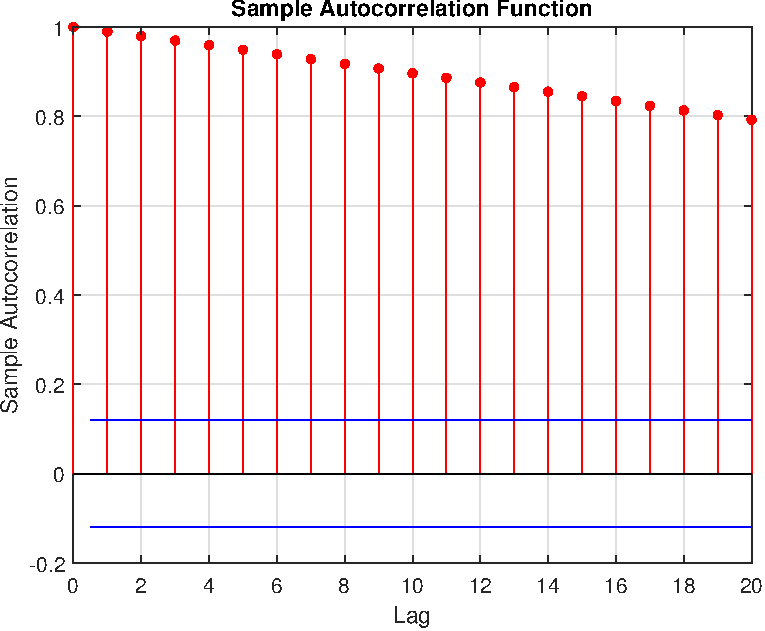
\includegraphics[width=.4\linewidth]{data-autocorrelation-plot.pdf}
  % \captionof{figure}{Question 4 - Autocorrelation plot of data}
  \label{fig:q4-data-autocorrplot}
\end{minipage}% Don't delete this comment - o.t. a spurious blank space will be added
\begin{minipage}{.5\textwidth}
  \centering
  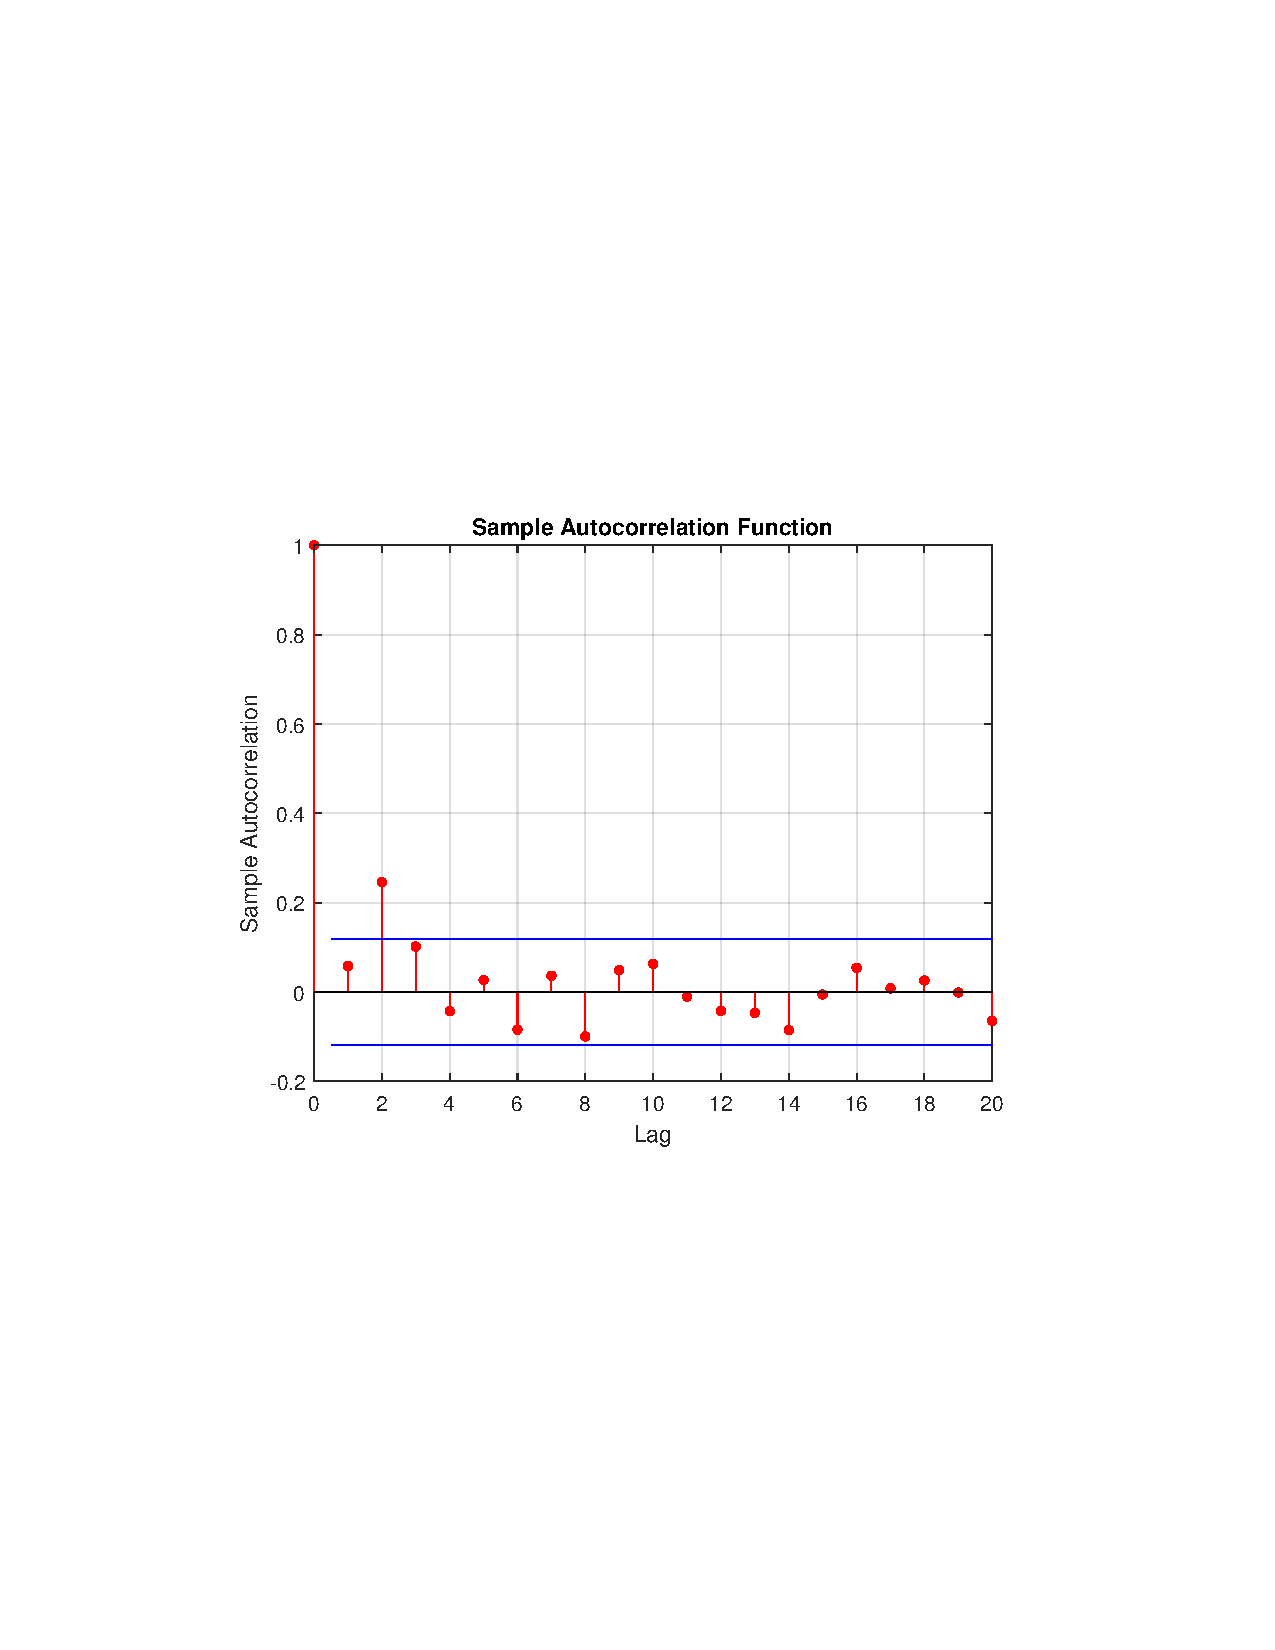
\includegraphics[width=.4\linewidth]{residual-autocorrelation-plot.pdf}
  % \captionof{figure}{Question 4 - Autocorrelation plot of residuals}
  \label{fig:q4-residual-autocorrplot}
\end{minipage}
\end{figure}

\begin{figure}[htp]
\centering
\begin{minipage}{.5\textwidth}
  \centering
  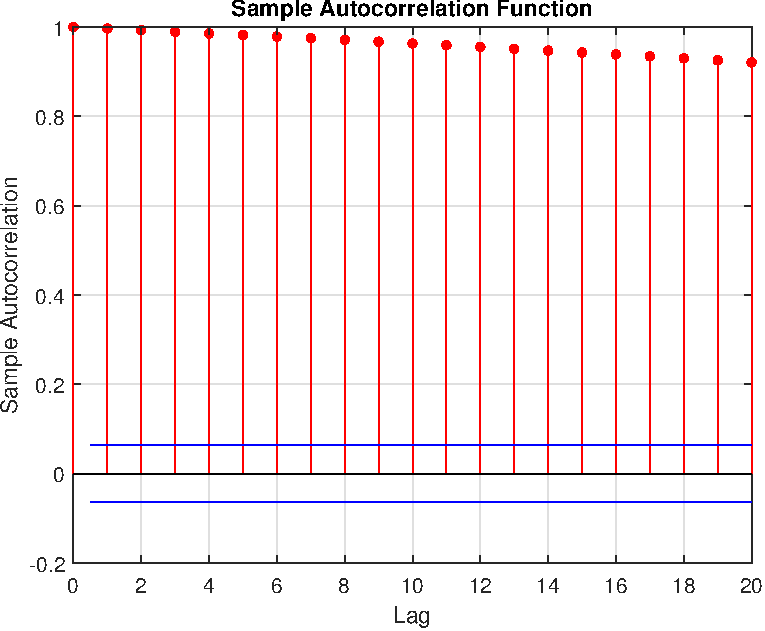
\includegraphics[width=.4\linewidth]{data-simulated-autocorrelation-plot.pdf}
  \captionof{figure}{Question 4 - Autocorrelation plot of simulated data}
  \label{fig:q4-data-simulated-autocorrplot}
\end{minipage}% Don't delete this comment - o.t. a spurious blank space will be added
\begin{minipage}{.5\textwidth}
  \centering
  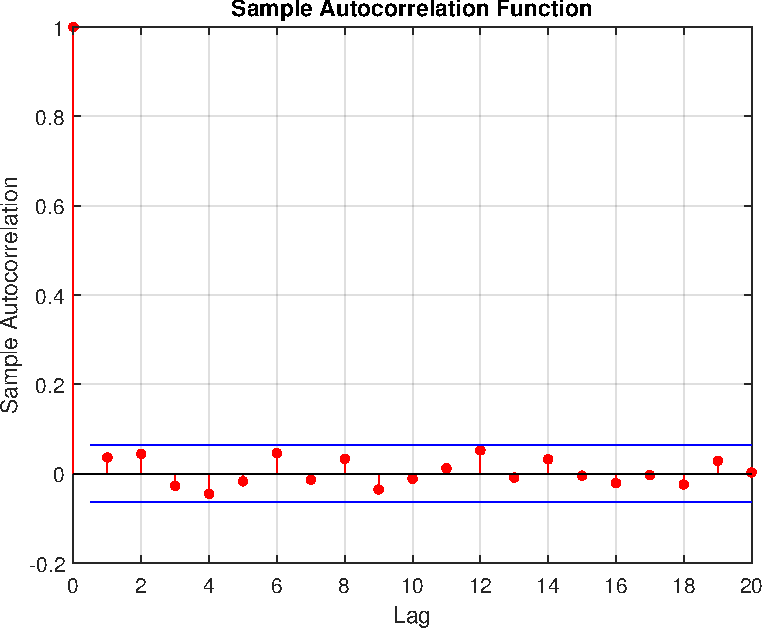
\includegraphics[width=.4\linewidth]{residual-simulated-autocorrelation-plot.pdf}
  \captionof{figure}{Question 4 - Autocorrelation plot of simulated residuals}
  \label{fig:q4-residual-simulated-autocorrplot}
\end{minipage}
\end{figure}

The model fits reasonably well. Firstly, the value of the value of the autoregressive coefficient in \ref{lst:data-output} is highly significant (with a p-value near 0 even), along with strong significance in the constant and variance. The R squared is \( 0.999857 \) (with the adjusted R being very similar since we are only estimating one lag) suggesting that the model explains the data very well. We also do a rudimentary test to see if the error is white noise in \ref{lst:resid-output} which shows that we cannot reject the null hypothesis at the 5\% significance that residuals have an AR(1) structure.

In figure \ref{fig:q4-data-autocorrplot} we see that the data clearly has a lagged structure. It is to be expected that with an AR(1) with a value for \( \rho \) close to 1, the lagged effects of the shock should be persistent. That is, we should {\itshape expect} non-zero auto correlation at all lags, which is in contrast to, say, an MA(q) process which only has non-zero autocorrelation for the first \( q \) lags. 

The autocorrelations of the residual of the above model are plotted in figure \ref{fig:q4-residual-autocorrplot}. This figure shows that most of the lags are within the confidence intervals around 0 and hence looks reasonably like white noise.

To verify our intuitions, we simulate an AR model with the same sample moments as the data in figures \ref{fig:q4-data-simulated-autocorrplot} and \ref{fig:q4-residual-simulated-autocorrplot}. Both confirm our findings that the data fits an AR(1) reasonably well.

There are some minor discrepancies when considering the Box-Ljuyng test that are persistent even with more lags. Despite that, we still believe that given the evidence that an AR(1) for consumption is a {\itshape reasonable} model.

\newpage
Next, consider the following economy.
\begin{align*}
\max & E_0 \sum^\infty_{t = 0}\beta^t \ln (c_t)\\
\intertext{subject to}
z_t A_t^{1 - \theta} k_t^\theta + (1 - \delta)k_t &= c_t + k_{t + 1}\\
A_t &= (1 + \gamma)^t, \quad t = 0, 1, \ldots \\
\ln(z_t) &= \rho \ln (z_{t - 1}) + \varepsilon_t,\quad \varepsilon_t \sim \mathcal{N}(0, \sigma^2_\varepsilon)
\end{align*}

Assume that the time period is annual. Construct a detrended version of
this economy and show the first order conditions. Choose $\beta$ so that the return
to capital in the steady state of the detrended economy is five percent, choose
$\theta$ so that capital’s share of income is 30 percent, and choose a depreciation rate
such that the share of investment to GDP in the steady state is 20 percent.
Choose $\rho = 0.95$, $\sigma^2_\varepsilon
 = .002$ and $\gamma = 0.02$.

\begin{align}
\intertext{Rearranging terms, we have}
k_{t + 1} &= A_t^{1 - \theta} k_t^\theta + (1 - \delta) k_t - c_t\\
Y_t &= A_t^{1 - \theta} k_t^\theta\\
c_t &= (1 - \theta) A_t^{1 - \theta} k_t^\theta\\
\intertext{To detrend, divide by $A_t$. Let's define a few new variables,}
\hat{k}_t &= \frac{K_t}{A_t}\\
\hat{y}_t &= \frac{Y_t}{A_t}\\
\hat{c}_t &= \frac{C_t}{A_t}.\\
\intertext{Now, we can substitute these back into the original equations.}
A \hat{k}_{t + 1} &= \hat{y}_t + (1 - \delta) \hat{k}_t - \hat{c}_t\\
1 + \gamma \hat{k}_{t + 1} &= \hat{y}_t + (1 - \delta) \hat{k}_t - \hat{c}_t\\
\hat{y}_t &= k^\theta\\
\hat{c}_t &= (1 - \theta) \hat{y}_t.\\
\intertext{First order conditions give us}
\frac{1}{\hat{c}_t} &= \frac{\beta}{1 + \gamma} E_t \left\{\frac{1}{\hat{c}_{t + 1}}\left[\frac{\theta \hat{y}_{t + 1}}{\hat{k}_{t + 1}} + 1 - \delta \right]\right\}.\\
\intertext{In the steady state, we have}
\frac{\overline{c}}{\overline{y}} &= \frac{1 + \gamma - \beta(1 - \delta) - \theta \beta (1 + \gamma - 1 + \delta)}{1 + \gamma - \beta (1 - \delta)}.\tag{$\ast$}\label{consumption-share}\\
\intertext{Now let's solve for parameters. We're given $\gamma = 0.02$, and we have to figure out $\beta$, $\theta$ and $\delta$. Since we have Cobb Douglas production, $\theta = 0.3$. To solve for $\beta$, note that the 5\% return implies}
\beta &= \frac{1}{1.05}\\
&= 0.95238.\\
\intertext{To solve for $\delta$, we're going to use equation \ref{consumption-share}. We're told that investment in the steady state is 20\% of GDP, so that implies that consumption is 80\% of GDP,}
0.8 &= \frac{1.02 - 0.95238(1 - \delta) - 0.3 \cdot 0.95238 (1.02 - 1 + \delta)}{1.02 - 0.95238 (1 - \delta)}\\
\implies \delta &= .082.
\end{align}

\newpage
\item 
 Log-linearize this model around its deterministic steady state. (For simplicity, assume that $z$ in the steady state is 1).

% \begin{align*}
% \max &E_0 \sum^\infty_{t = 0} \beta^t \ln (c_t)\\
% \text{s.t. } c_t + i_t &\le y_t \\
% i_t &= k_{t + 1} - (1 - \delta) k_t \\
% y_t &= z_t A^{1 - \theta}_t k^\theta_t \\
% A_t &= (1 + \gamma)^t \\
% \ln (z_t) &= \rho \ln (z_{t - 1}) + \varepsilon_t \\
% \varepsilon_t &\sim \mathcal{N}(0, \sigma^2_\varepsilon)\\
% \intertext{Set up the recursive problem:}
% V(K_t, z_{t - 1}) &= \ln (c_t) + \beta E[V(K_t, z_t) \mid z_{t - 1}]\\
% \text{s.t. } K_{t + 1} &= (1 - \delta)K_t + y_t - c_t \\
% y_t &= z_t A_t^{1 - \theta}K_t^\theta \\
% \ln (z_t) &= \rho \ln (z_{t - 1})\\
% \intertext{Take first order conditions:}
% \frac{1}{c_t} &= \lambda \\
% \beta E[V'(K_{t + 1}, z_t) \mid z_{t - 1}] &= \lambda \\
% \implies \frac{1}{c_t} &= \beta E [V'(K_{t + 1}, z) \mid z_{t - 1}]\\
% V'(K_t, z_{t - 1}) &= \frac{1}{c_t} (\theta z_t A_t^{1 - \theta}K_t^{\theta - 1} + 1 - \delta)\tag{Envelope}\\
% \frac{c_{t + 1}}{c_t} &= \beta E [\theta z_{t + 1} A^{1 - \theta}_{t + 1}K^{\theta - 1}_{t + 1} + 1 - \delta]\\
% \intertext{Define some new variables \ldots}
% \hat{K}_t &\equiv \frac{K_t}{A_t}\\
% \hat{c}_t &\equiv \frac{c_t}{A_t}\\
% \hat{y}_t &\equiv \frac{y_t}{A_t}\\
% \intertext{Now substitute these new variables into our old equations:}
% k_{t + 1} &= (1 - \delta)K_t + y_t - c_t \tag{old}\\
% \implies \hat{K}_{t + 1} A &= (1 - \delta) \hat{K}_t + \hat{c}_t - \hat{c}_t\\
% y_t &= z_t A^{1 - \theta}_t k^\theta_t \tag{old}\\
% \implies \hat{y}_t &= z_t \hat{k}_t^\theta \\
% \frac{c_{t + 1}}{c_t} &= \beta E[\theta z_{t + 1}A^{1 - \theta}_{t + 1}K^{\theta - 1}_{t + 1} + 1 - \delta] \tag{old}\\
% \implies \frac{\hat{c}_{t + 1}}{\hat{c}_t} &= \frac{\beta}{A} E[\theta z_{t + 1}\hat{K}^{\theta - 1}_{t + 1} + 1 - \delta]
% \end{align*}

\begin{align*}
\text{Define } \tilde{x} &\equiv \log\left(\frac{\hat{x}}{\overline{x}}\right).\\
\intertext{From the Euler equation, we have}
\frac{\hat{c}_{t + 1}}{\hat{c}_t} &= \frac{\beta}{A} E_t [\theta z_{t + 1}\hat{K}^{\theta - 1}_{t + 1} + 1 - \delta].\\
\intertext{Substituting our log linearization into the left-hand side, we have}\\
\frac{\overline{c}\exp(\tilde{c}_{t + 1})}{\overline{c} \exp (\tilde{c}_t)} &\approx (1 + \tilde{c}_{t + 1})(1 - \tilde{c}_t)\tag{LHS}\\
&\approx 1 + \tilde{c}_{t + 1} - \tilde{c}_t \tag{LHS}.\\
\intertext{Doing the same thing on the right-hand side, we have}
\frac{\beta}{A} E_t [\theta \overline{z} (1 + \tilde{z}_{t + 1})\overline{K}(1 + (\theta - 1)\hat{K}_{t + 1}) + 1 - \delta] &=
\frac{\beta}{A} E_t [\theta \overline{z} \overline{K}^{\theta - 1}(\theta - 1)\tilde{K}_{t + 1} + \theta \overline{z} \overline{K}^{\theta - 1}\tilde{z}_{t + 1} + 1 - \delta]\\
\intertext{In the steady state,}
1 &= \frac{\beta}{A}(\theta \overline{z} \overline{K}^{\theta - 1} + 1 - \delta),\\
\overline{z} &= 1.\\
\intertext{We can use these to simplify the log-linearized Euler equation:} 
\tilde{c}_{t + 1} - \tilde{c}_t &= \frac{\beta}{A} E_t [\theta \overline{K}^{\theta - 1}(\theta - 1)\tilde{K}_{t + 1} + \theta \overline{K}^{\theta - 1} \tilde{z}_{t + 1}].\\
\intertext{Now, let's do the same thing to the budget constraint.}
\hat{c}_t + A\hat{K}_{t + 1} &= z_t \hat{K}_t^\theta + (1 - \delta)\hat{K}_t \\
\overline{c}(1 + \tilde{c}_t) + A \overline{K} (1 + \hat{K}_{t + 1}) &= \overline{c} + A\overline{K} + \overline{c}\tilde{c}_t + A\overline{K}\tilde{K}_{t + 1}\tag{LHS}\\
\overline{z}(1 + \tilde{z}_t)\overline{K}^\theta (1 + \theta \tilde{K}_t) + (1 - \delta)\overline{K}(1 + \tilde{K}_t) &=
\overline{z} \overline{K}^\theta + \overline{z} \overline{K}^\theta \theta \tilde{K}_t + \overline{z} \overline{K}^\theta \tilde{z}_t + (1 - \delta) \overline{K} + (1 - \delta)\overline{K} \tilde{K}_t \tag{RHS}.\\
\intertext{In the steady state,}
\overline{c} + A \overline{K} &= \overline{z}\overline{K}^\theta + (1 - \delta)\overline{K},\\
\overline{z} &=1,
\intertext{so we can simplify this expression to}
\overline{c}\tilde{c}_t + A\overline{K}\tilde{K}_{t + 1} &= \overline{K}^\theta \theta \tilde{K}_t + \overline{K}^\theta \tilde{z}_t + (1 - \delta)\overline{K}\tilde{K}_t,\\
\intertext{or}
\tilde{k}_{t + 1} &= \frac{\overline{K}^{\theta - 1}}{A} \theta \tilde{K}_t + \frac{\overline{K}^{\theta - 1}}{A} \tilde{z}_t + \frac{1 - \delta}{A}\hat{K}_t - \frac{\overline{c}}{A \overline{K}} \tilde{c}_t.\\
\intertext{Finally, for the stochastic process, }
\ln (z_t) &= \rho \ln (z_{t - 1}) + \varepsilon_t\\
\ln (\overline{z}\exp(\tilde{z}_t)) &= \rho \ln (\overline{z} \exp(\tilde{z}_{t - 1})) + \varepsilon_t\\
\ln (\overline{z}) + \tilde{z}_t &= \rho \ln (\overline{z}) + \rho \tilde{z}_{t - 1} + \varepsilon_t \\
\implies \tilde{z}_t &= \rho \tilde{z}_{t - 1},\\
\intertext{or}
\tilde{z}_{t + 1}&= \rho \tilde{z}_t.\\
\end{align*}
\begin{align*}
\intertext{Putting everything together, the log-linearized version of this economy is}
\tilde{c}_{t + 1} &= E_t \left\{\frac{\beta \theta \overline{K}^{\theta - 1}}{A}(\theta - 1)\left[\frac{\theta \overline{K}^{\theta - 1} + 1 - \delta}{A}\tilde{K}_t + \frac{\overline{K}^{\theta - 1}}{A}\tilde{z}_t - \frac{\overline{c}}{A \overline{K}} \tilde{c}_t\right]\right\}\\
\hat{k}_{t + 1} &= \frac{\theta \overline{K}^{\theta - 1} + 1 - \delta}{A} \hat{K}_t + \frac{\overline{K}^{\theta - 1}}{A} \tilde{z}_t - \frac{\overline{c}}{A \overline{K}}\tilde{c}_t\\
\tilde{z}_{t + 1} &= \rho \tilde{z}_t.
\end{align*}

\newpage
\item Use the formula of Blanchard and Kahn to show that there is a unique
stationary solution to the linearized system.

\newpage
\item Using a random number generator (Matlab has a built-in function for
this), draw 1100 values of $\varepsilon$ to construct the $z$ process. Using these values of $z$,
and assuming that $k_0$ is equal to its steady state value, use the linearized system
to construct 1100 values values of output, consumption, and investment.

\begin{align}
\intertext{I'm having some trouble with this question. I'm not sure if I'm doing something dumb, but I started with Ben's linearized equations and didn't know how to treat $\overline{k}$. The problem says that $k_0 = \overline{k}$, so $\tilde{k}$ should be zero, but $\overline{k}$ was in a bunch of other terms so here's what I've got so far. From earlier in the problem, we have}
\overline{K}^{\theta - 1} &= \frac{\beta \theta \overline{z}}{A - \beta (1 - \delta)}.\\
\intertext{Substituting this into the expression for $\tilde{K}_{t + 1}$ gives}
\tilde{k}_{t + 1} &= \left[\theta \cdot \left(\frac{\beta \theta \overline{z}}{A - \beta (1 - \delta)}\right) + 1 - \delta \right] \cdot A^{-1} \cdot \tilde{k_t} + \left(\frac{\beta \theta \overline{z}}{A - \beta(1 - \delta)}\right) \cdot A^{-1} \cdot \tilde{z}_t - \underbrace{\frac{\overline{c}}{A \overline{K}}}_{\text{simplify}} \tilde{c}_t\\
\intertext{To simplify this last term, start with}
\overline{c} &= \overline{y} + (1 - \delta - A)\overline{k}\overline{k}\\
\implies \frac{\overline{c}}{\overline{K}} &= \frac{\overline{y} + (1 - \delta - A)\overline{K}}{\overline{K}}\\
&= \frac{\overline{y}}{\overline{K}} + 1 - \delta - A\\
\frac{\overline{y}}{\overline{K}} &= \frac{\overline{K}}{\overline{Y}} \cdot 1^{-1}\\
 &= \frac{A - \beta (1 - \delta)}{\beta \theta \overline{z}}\\
\implies \frac{\overline{c}}{\overline{K}} &= \left(\frac{A - \beta (1 - \delta)}{\beta \theta \overline{z}} + 1 - \delta - A\right)\\
\intertext{Putting this all together, the computationally tractable form of $\tilde{k}_{t + 1}$ should be }
\tilde{k}_{t + 1} &= \left[\theta \cdot \left(\frac{\beta \theta \overline{z}}{A - \beta (1 - \delta)}\right) + 1 - \delta \right] \cdot A^{-1} \cdot \tilde{k_t}\\ &\hspace{4em} + \left(\frac{\beta \theta \overline{z}}{A - \beta(1 - \delta)}\right) \cdot A^{-1} \cdot \tilde{z}_t \\ &\hspace{4em} - \left(\frac{A - \beta (1 - \delta)}{\beta \theta \overline{z}} + 1 - \delta - A \right) \cdot A^{-1} \cdot \tilde{c}_t\\
\intertext{$\overline{z}$ is 1, and everything else is a parameter except for the tilde variables, so this should work (I dropped $t$ subscripts on $A$ but that should be fine). I think this all looks okay but I'm not sure if there was an easier way to do this? If we do the same thing for consumption,}
\tilde{c}_{t + 1} &= E_t \left\{\frac{\beta \theta \overline{K}^{\theta - 1}}{A} \cdot (\theta - 1) \tilde{k}_{t + 1}\right\}\\
&= E_t \left\{\beta \theta \cdot \left(\frac{\beta \theta \overline{z}}{A - \beta (1 - \delta)}\right)\cdot \frac{\theta - 1}{A} \cdot \tilde{c}_{t + 1}\right\}\\
&= \beta \theta \cdot \left(\frac{\beta \theta \overline{z}}{A - \beta (1 - \delta)}\right) \cdot \frac{\theta - 1}{A} \cdot E_t\left\{\tilde{k}_{t + 1}\right\}\\
\intertext{I'm a bit confused about this expectation, because it's taken at time $t$ and all the terms in $\tilde{k}_{t + 1}$ have $t$ subscripts, so shouldn't they be known? But I thought that consumers chose their consumption based on the expected next-period shock. One last thing that I'm pretty sure is me being dumb/lazy, but it seems like I need to use $\tilde{k}$ to calculate $k$ in order to get $y$ and $i$ and solve the problem. Is there a straightforward way to do this? }
\tilde{k} &\equiv \log \left(\frac{\hat{k}}{\overline{k}}\right)\\
e^{\tilde{k}} &= \frac{\hat{K}}{\overline{K}}\\
&= \frac{K_t}{\overline{K}A_t}\\
\intertext{Do we have a nice expression/number for $\overline{K}$, or do I have to solve for this using an approach from Gary's half of the class?}
\end{align}

\newpage
\item Discard the first 100 observations, and then fit an AR(1) process to the
log of consumption, measured as the log-deviation of consumption from the
steady state value. Report the value of the AR(1) coefficient in the regression,
and evaluate whether there is autocorrelation in the residuals.

\newpage
\item Compare the regression coefficient in (9) and your assessment of the
autocorrelation in the residuals, to your answers in (4) and (5). Does the RBC
model provide a good approximation to consumption dynamics? What does it
tell us about using consumption data to try to discriminate between the Hall
\end{enumerate}
\end{document}
